\scanpage{41}
\uline{Remarque} \deleted{\unsure{Supp}} Soit $\unsure{B|S}$ \inserted{$=\operatorname{Spec}R$} un schéma local noeth complet, $\mathfrak X$ un schéma formel propre \deleted{et} plat sur $S$, tel que $H^0(X_0,\mathcal O_{X_0})\simeq k$ (pour simplifier). Supposons aussi \deleted{\unsure{que}} que \deleted{$\underline{\operatorname{Pic}}^0_{X_0/k}$ soit lisse, soit que} les $\underline{\operatorname{Pic}}^0_{X_n/S_n}$ soient plats \deleted{soit que} \inserted{(p.ex. $\underline{\operatorname{Pic}}^0_{X_0/k}$ lisse)}, de sorte qu'on peut former
\[
\underline{NS}_{X_n/S_n}=\underline{\operatorname{Pic}}_{X_n/S_n}/\underline{\operatorname{Pic}}^0_{X_n/S_n},
\]
et les sous-schémas
\[
P_n=\underline{NS}^{+}_{X_n/S_n}\quad\text{(partie ample).}
\]
Les $P_n$ sont nets sur les $S_n$, et par recollement définissent un schéma formel $\widehat P$ sur $\widehat S$, tel que
\[
\widehat P=\coprod_\alpha\widehat P_\alpha
\]
les $P_\alpha$ étant finis \inserted{nets} sur $S$ et connexes. Procédant comme plus haut, on trouve que les conditions suivantes sont équivalentes

(i) $\exists\ S'\longrightarrow S$ \uline{propre} surjectif, \inserted{\deleted{\unsure{plat}}} avec $\widehat X_{\widehat S'}$ algébrique et \uline{projectif} sur $S'$.

(ii) $\forall$ sous-schéma fermé \inserted{$T$ de $S$} de dim $\leq1$, si $T'$ est son normalisé, alors $\widehat X_{\widehat T'}$ est algébrique et projectif sur $\widehat T'$.

(iii) $\exists$ morphisme \inserted{fini} surjectif net $S'\mathbin{-}S$, tel que $\widehat X_{\widehat S'}$ soit algébrique et projectif.

\margin{\figure{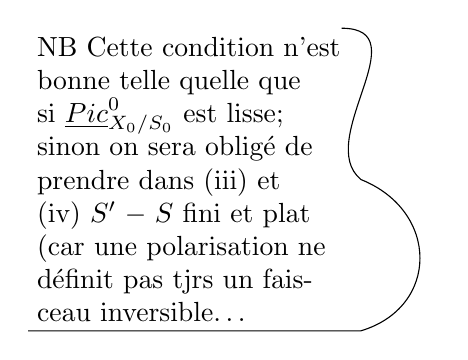
\begin{tikzpicture}\node[align=left,text width=4cm,inner sep=3pt](m){\uline{NB} Cette condition n'est bonne telle quelle que si $\underline{\operatorname{Pic}}^0_{X_0/S_0}$ est lisse; sinon on \unsure{sera} obligé de prendre \inserted{dans (iii) et (iv)} $S'\mathbin{-}S$ \uline{fini et plat} (car une polarisation ne définit pas tjrs un \unsure{faisceau} \unsure{inversible}$\ldots$};\draw ([xshift=-7pt]m.north east) .. controls +(1,0) and +(-.6,.5) .. (m.east) .. controls +(1,-.4) and +(1,.3) .. (m.south east) -- (m.south west);\end{tikzpicture}}}

(iv) Il existe un morphisme fini étale surjectif $S'\longrightarrow S$, tel que pour tte composante irréductible $S'_i$ de $S'$, avec str. réduite induite, $\widehat X_{\widehat S'_i}$ est rationnellement projectif.

\deleted{Ces conditions \unsure{sont} \unsure{équivalentes} \unsure{à} \unsure{l'algébricité} \unsure{de} $\unsure{\widehat X}$.}
De plus, si $S'\longrightarrow S$ est comme dans (iv), $\widehat X_{\widehat S'}$ est algébrique.
\deleted{\unsure{Alors} $(iii)$ $\exists$ \unsure{morphisme} \unsure{fini} \unsure{plat} \unsure{surjectif}}

\margin{$*$ \unsure{on} \unsure{démontre} \unsure{leur} d'ailleurs \unsure{effectivité|affinité}.}

\figure{\begin{tikzpicture}\draw (0,1.2)--(.1,0)--(.4,-.03);\end{tikzpicture}}
\mspage{40}
